\documentclass[mathserif]{beamer}

\usetheme{Boadilla}

\usepackage{subfig}

% Chinese
\usepackage{ctex}
\setCJKmainfont[BoldFont={SimHei},ItalicFont={KaiTi}]{KaiTi}

% Title
\title{第4章 实验建模}
\author{韩建伟}
\institute{
  浙江工商大学信息学院\\
  \texttt{hanjianwei@mail.zjgsu.edu.cn}
}
\date{2011/10/10}

\begin{document}

% Title page
\begin{frame}[plain]
  \titlepage{}
\end{frame}

\begin{frame}{拟合和插值的选择}

  \begin{description}
  \item[拟合] 建模者利用一些假定来选择一个特定的模型类型,以解释观测值反应的状况.
  \item[插值] 建模者不可能构造一个满意地解释已知状况的易于处理的模型.
  \end{description}

  \begin{figure}
    \centering
    \subfloat[数据]{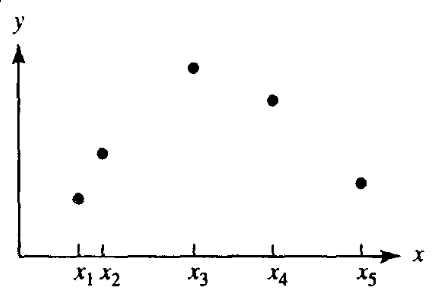
\includegraphics[height=.3\textheight{}]{data.png}}
    \subfloat[拟合]{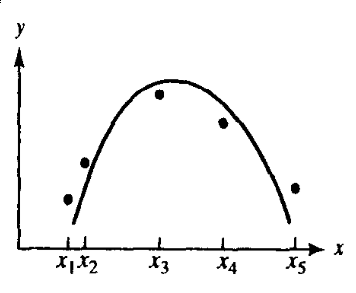
\includegraphics[height=.3\textheight{}]{fit.png}}
    \subfloat[插值]{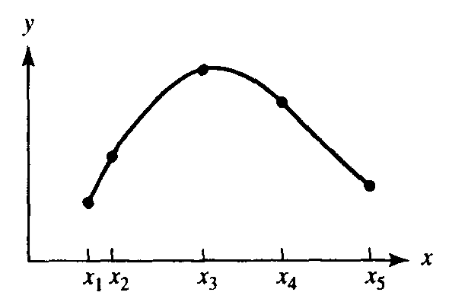
\includegraphics[height=.3\textheight{}]{interpolate.png}}
  \end{figure}

\end{frame}

\begin{frame}{Chesapeake海湾的收成}

  \begin{figure}
    \centering
    \setcounter{subfigure}{0}{}
    \subfloat[收成数据]{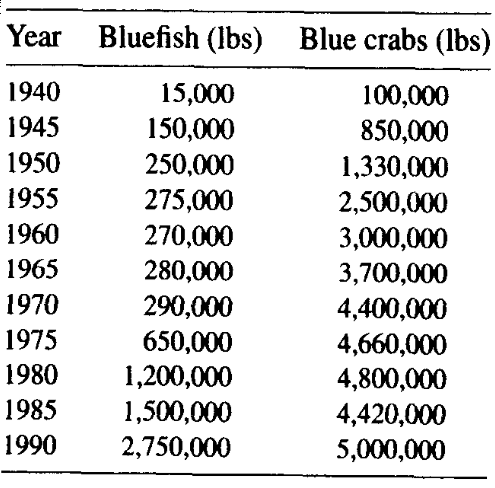
\includegraphics[height=.28\textheight{}]{harvest.png}}
    \subfloat[蓝鱼散点图]{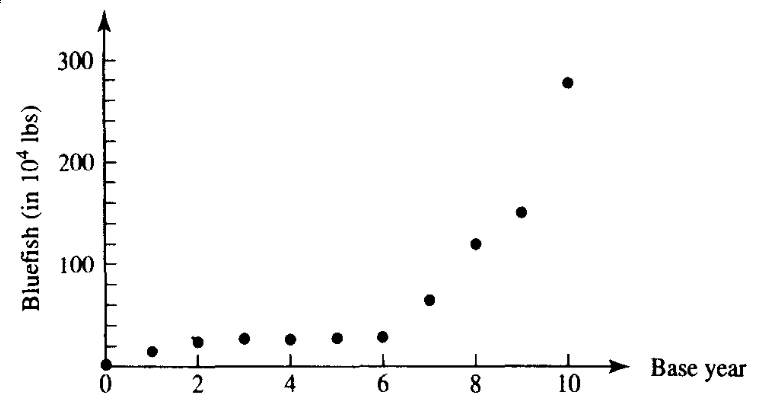
\includegraphics[height=.28\textheight{}]{bluefish-plot.png}}
    \subfloat[蓝蟹散点图]{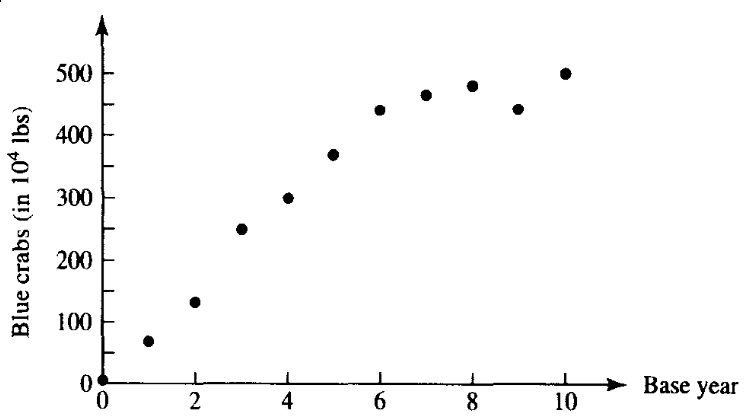
\includegraphics[height=.28\textheight{}]{bluecrab-plot.png}}
    \caption{1992年《每日评论》收集的过去50年中Chesapeake海湾的海产收成.}
  \end{figure}
  
\end{frame}

\begin{frame}{如何对数据进行变换}

  \begin{figure}
    \centering
    \setcounter{subfigure}{0}{}
    \subfloat[三种变换]{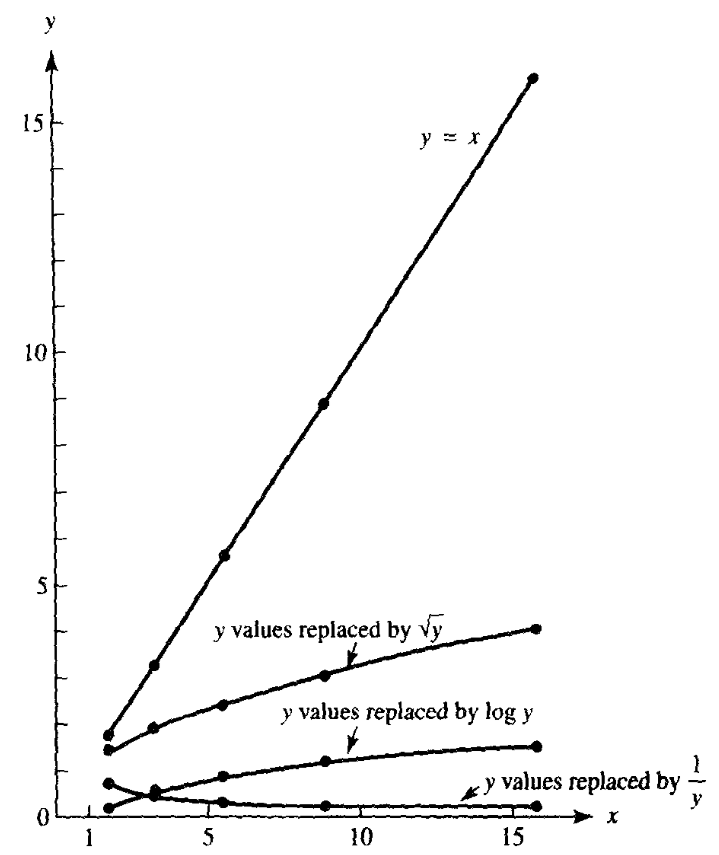
\includegraphics[height=.6\textheight{}]{transform.png}}
    \subfloat[变换阶梯]{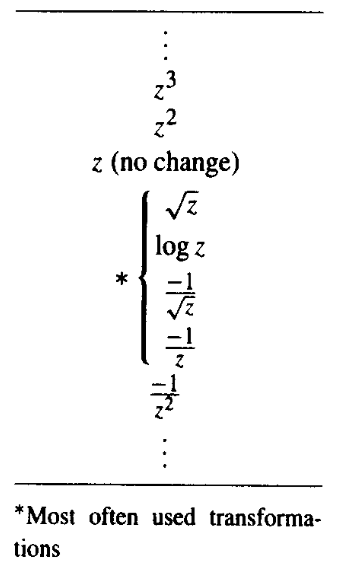
\includegraphics[height=.6\textheight{}]{ladder.png}}
  \end{figure}

  \begin{center}
    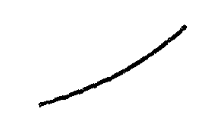
\includegraphics[height=.1\textheight{}]{down.png}
    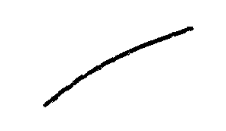
\includegraphics[height=.1\textheight{}]{up.png}
  \end{center}
  
\end{frame}

\begin{frame}{收获蓝鱼}

  \begin{itemize}
  \item “向下压”曲线的右端,用最小二乘法拟合下列模型:
    \[
    \log y = mx + b
    \]
  \end{itemize}

  \begin{figure}
    \centering
    \setcounter{subfigure}{0}{}
    \subfloat[蓝鱼数据]{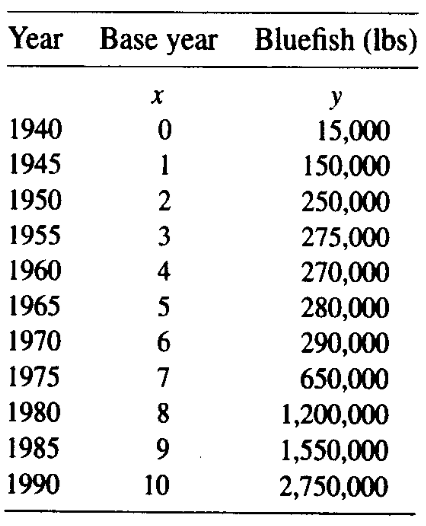
\includegraphics[height=.4\textheight{}]{bluefish.png}}
    \subfloat[蓝鱼拟合$y=5.457(1.4635)^x$]{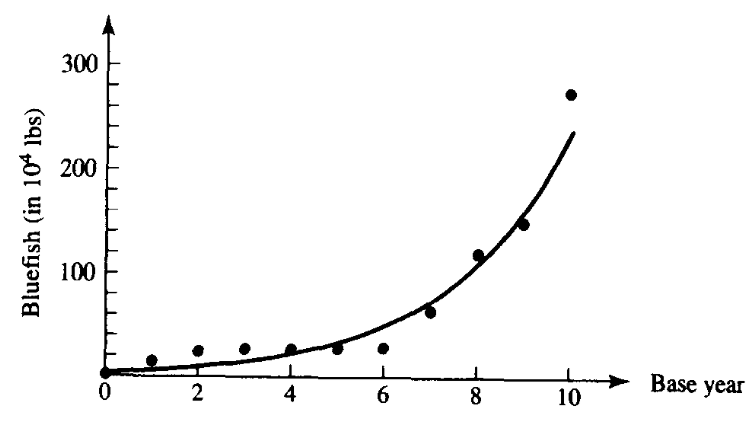
\includegraphics[height=.4\textheight{}]{bluefish-fit.png}}
  \end{figure}
  
\end{frame}

\begin{frame}{收获蓝蟹}

  \begin{itemize}
  \item “向上扳”曲线的右端,用最小二乘法拟合下列模型:
    \[
    y = k\sqrt{x}
    \]
  \end{itemize}

  \begin{figure}
    \centering
    \setcounter{subfigure}{0}{}
    \subfloat[蓝蟹数据]{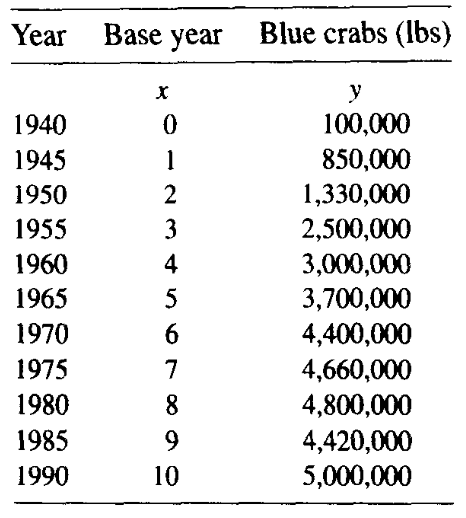
\includegraphics[height=.4\textheight{}]{bluecrab.png}}
    \subfloat[蓝蟹拟合直线$y=158.344\sqrt{x}$]{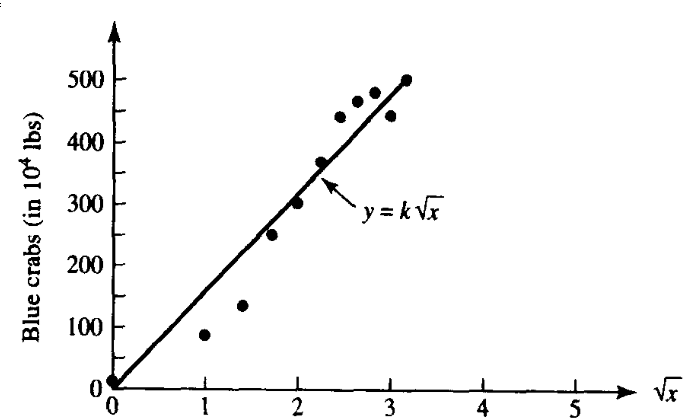
\includegraphics[height=.4\textheight{}]{bluecrab-line.png}}
  \end{figure}
  
\end{frame}

\begin{frame}{蓝蟹最终拟合数据}

  \begin{figure}
    \centering
    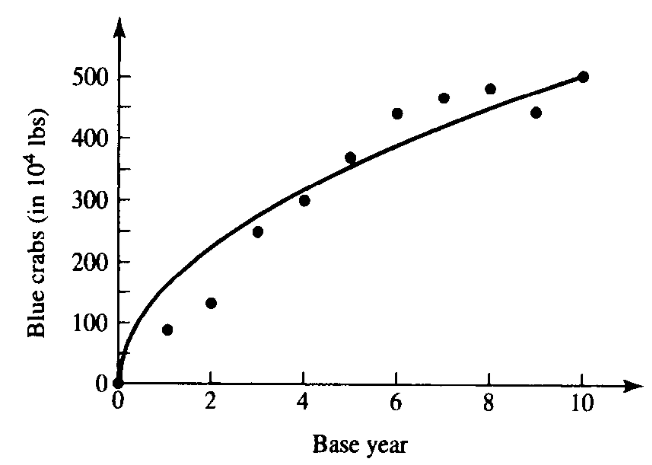
\includegraphics[height=.6\textheight{}]{bluecrab-fit.png}
  \end{figure}
  
\end{frame}

\begin{frame}{验证模型}

  \begin{itemize}
  \item 针对每一对数据,计算残差和相对误差.
  \item 对未来进行预测或者外推,这些模型是否依然适用.
  \item 这些简单的单项模型应该用于插值而不是外推.
  \end{itemize}
  
\end{frame}

\begin{frame}{本节的想法}


  构造一个模型时,从细心分析收集到的数据开始:
    \begin{enumerate}
    \item 看数据存在什么样的倾向
    \item 是否有明显处于倾向以外的点?如果有这样的异常值,想想是否抛弃它们?如果是实验观测到的,重复该实验做一个数据收集错误的检查.
    \item 当倾向确实清楚存在时,下一步是找到一个将数据变换成一(近似)直线的函数.
    \item 警惕变换的使用如何带来欺骗性,特别是当数据点集中在一起时.
    \item 最后,用第3章讨论的指示量分析拟合优度,记住对原始的而不是变换后的数据画出所提供的模型.
    \item 如果对这一拟合不满意,可以研究其它的单项模型.
    \end{enumerate}
  
\end{frame}

\begin{frame}{高阶多项式模型}

  \begin{itemize}
  \item 单项模型易于进行模型分析,包括敏感性分析、优化、变化率以及曲线下面积的估计.
  \item 单项模型的可用性有限.
  \item 解决方案:多项模型.
  \end{itemize}

  \begin{figure}
    \centering
    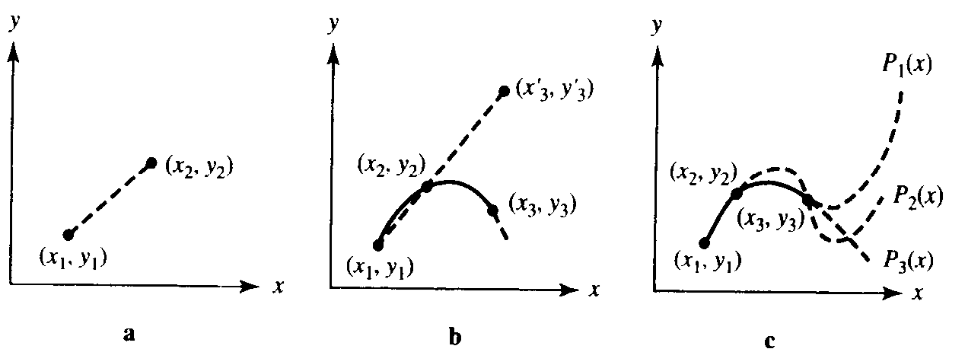
\includegraphics[width=.8\textwidth{}]{unique-poly.png}
    \caption{通过三个数据点且最高阶为2的多项式只有唯一一个,而阶高于2的多项式有无穷多个}
  \end{figure}
  
\end{frame}

\begin{frame}{录音机的播放时间}
  \begin{figure}
    \centering
    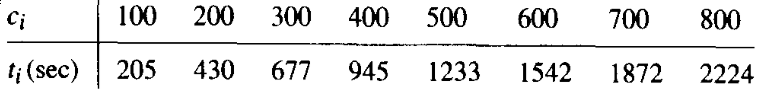
\includegraphics[width=.6\textwidth{}]{record-tab.png}
    \caption{录音机计数器和播放时间关系表}
  \end{figure}
  我们有8个数据点,应期望一个最高阶为7的唯一多项式,记为
  \[
  P_7(c) = a_0 + a_1c + a_2c^2 + a_3c^3 + a_4c^4 + a_5c^5 + a_6c^6 + a_7c^7
  \]
  把8个数据点代入
  \[
  205 = a_0 + a_11 + a_21^2 + a_31^3 + a_41^4 + a_51^5 + a_61^6 + a_71^7
  \]
  \[
  430 = a_0 + a_12 + a_22^2 + a_32^3 + a_42^4 + a_52^5 + a_62^6 + a_72^7
  \]
  \[
  \vdots
  \]
  \[
  2224 = a_0 + a_18 + a_28^2 + a_38^3 + a_48^4 + a_58^5 + a_68^6 + a_78^7
  \]
\end{frame}

\begin{frame}{系数求解}

  \begin{figure}
    \centering
    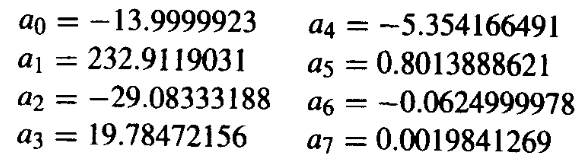
\includegraphics[width=.4\textwidth{}]{record-sol.png}
  \end{figure}

  \begin{figure}
    \centering
    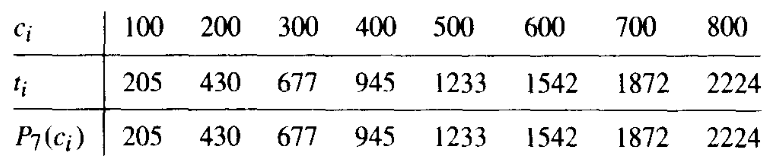
\includegraphics[width=.7\textwidth{}]{record-comp.png}
  \end{figure}

  考虑第3章提出的评判标准...该模型真的是最好的吗?
  
\end{frame}

\begin{frame}{多项式的拉格朗日形式}

  \begin{block}{定理1}
    如果$x_0$,$x_1$,...,$x_n$是$n+1$个不同的点,而$y_0$,$y_1$,...,$y_n$是这些点上对应的观测值,那么,存在一个唯一的最高阶为$n$的多项式$P(x)$,具有性质
    \[
    y_k = P(x_k), k = 0, 1, ..., n
    \]
    这一多项式由下式给定
    \[
    P(x) = y_0L_0(x) + ... + y_nL_n(x)
    \]
    其中
    \[
    L_k(x) = \frac{(x-x_0)(x-x_1)...(x-x_{k-1})(x-x_{k+1})...(x-x_n)}{(x_k-x_0)(x_k-x_1)...(x_k-x_{k-1})(x_k-x_{k+1})...(x_k-x_n)}
    \]

  \end{block}
  
\end{frame}

\begin{frame}{高阶多项式的优缺点}
  \begin{block}{缺点1}
    在端点附近多项式有严重摆动, 进行数据预测时有很大问题
  \end{block}
  
  \begin{figure}
    \centering
    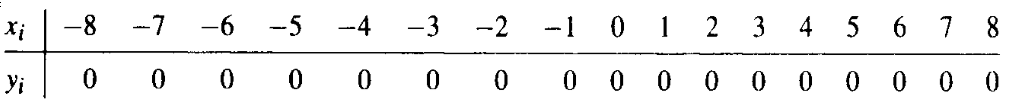
\includegraphics[width=.8\textwidth{}]{highorder-tab.png}
  \end{figure}
  \begin{figure}
    \centering
    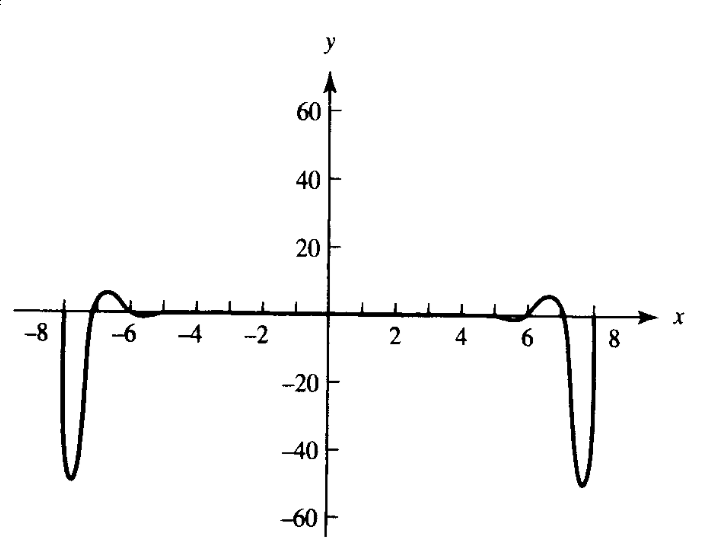
\includegraphics[width=.5\textwidth{}]{highorder-fig.png}
  \end{figure}
  
\end{frame}

\begin{frame}{高阶多项式的优缺点}
  \begin{block}{缺点2}
    对数据微小变换非常敏感
  \end{block}

  \begin{figure}
    \centering
    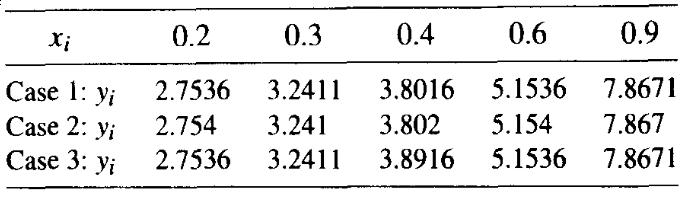
\includegraphics[width=.4\textwidth{}]{small-tab.png}
    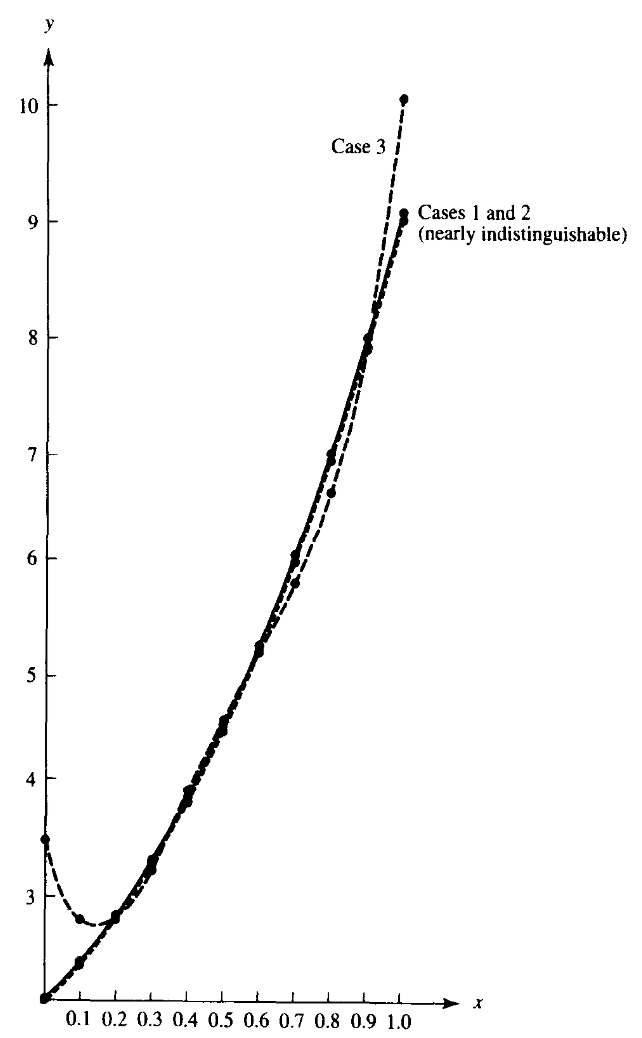
\includegraphics[height=.7\textheight{}]{small-fig.png}
  \end{figure}

\end{frame}

\begin{frame}{光滑化:低阶多项式模型}

  \begin{block}{光滑化}
    不管数据的个数, 选取一个低阶多项式,通过第3章的准则拟合给定的数据.
  \end{block}

  \begin{figure}
    \centering
    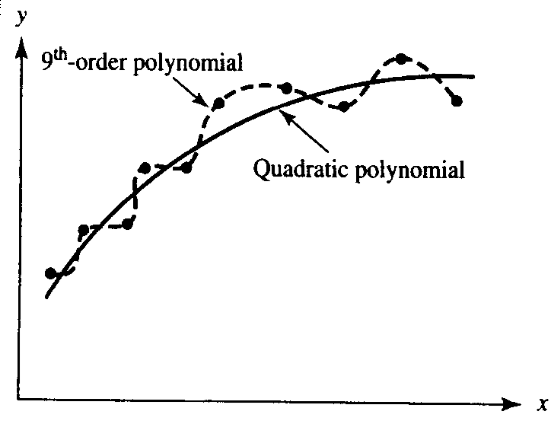
\includegraphics[width=.6\textwidth{}]{smooth.png}
  \end{figure}
  
\end{frame}

\begin{frame}{再论录音机的播放时间}

  \begin{figure}
    \centering
    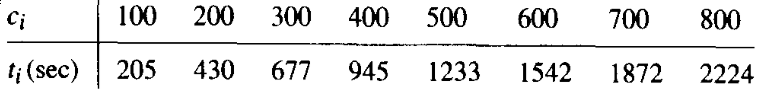
\includegraphics[width=.6\textwidth{}]{record-tab.png}
    \caption{录音机计数器和播放时间关系表}
  \end{figure}

  拟合一个下列形式的二阶多项式
  \[
  P_2(c) = a + bc + dc^2
  \]

  用最小二乘法确定$a$, $b$, $c$.

\end{frame}

\begin{frame}{最小二乘法拟合}
  \[
  \text{Minimize } S = \sum_{i=1}^m [t_i - (a+bc_i+dc_i^2)]^2
  \]
  存在极小点的必要条件
  \[
  \frac{\partial S}{\partial a} = \frac{\partial S}{\partial b} = \frac{\partial S}{\partial d} = 0
  \]
  故
  \[
  ma + (\sum c_i)b + (\sum c_i^2)d = \sum t_i
  \]
  \[
  (\sum c_i)a + (\sum c_i^2)b + (\sum c_i^3)d = \sum c_it_i
  \]
  \[
  (\sum c_i^2)a + (\sum c_i^3)b + (\sum c_i^4)d = \sum c_i^2t_i
  \]
\end{frame}

\begin{frame}{拟合结果}
  \[
  P_2(c) = 0.14286 + 1.94226c + 0.00105c^2
  \]

  \begin{figure}
    \centering
    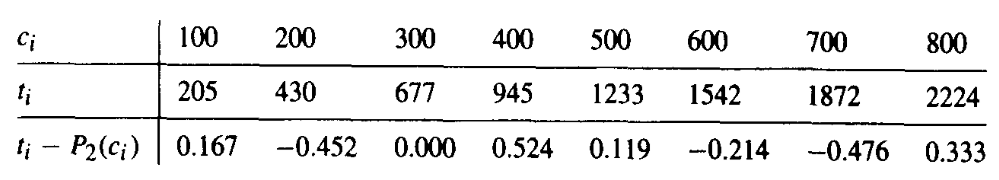
\includegraphics[width=.7\textwidth{}]{record-fit2.png}
  \end{figure}

  \begin{enumerate}
  \item 应该用一个多项式吗?
  \item 如果应该,几阶的多项式合适?
  \end{enumerate}
  
\end{frame}

\begin{frame}{多项式阶数的确定}
  \[
  P(x) = a + bx + cx^2
  \]
  \[
  P'(x) = b+2cx
  \]
  \[
  P''(x) = 2c
  \]
  \[
  P'''(x) = 0
  \]

\end{frame}

\begin{frame}{导数的离散形式}
  \[
  \frac{\mathrm{d}y}{\mathrm{d}x} = \lim_{\Delta x \rightarrow 0}\frac{\Delta y}{\Delta x}
  \]

  \begin{figure}
    \centering
    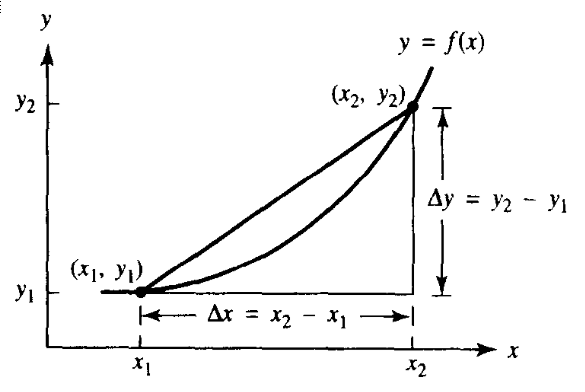
\includegraphics[width=.6\textwidth{}]{dif-fig.png}
  \end{figure}
  
\end{frame}

\begin{frame}{离散求导示例}
  \begin{figure}
    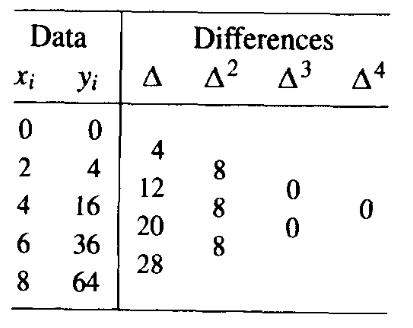
\includegraphics[width=.3\textwidth{}]{dif-sample.png}
  \end{figure}
  \begin{figure}
    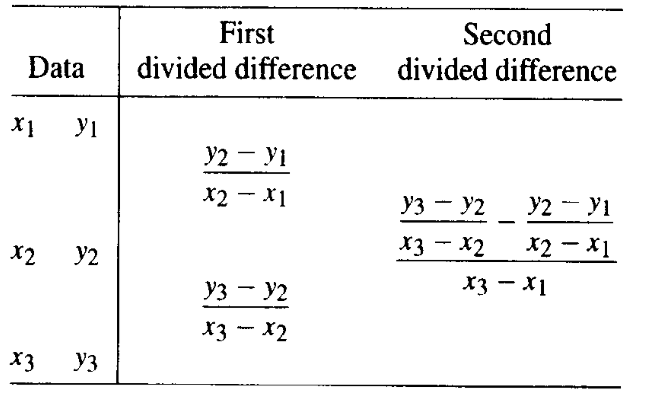
\includegraphics[width=.4\textwidth{}]{dif-tab.png}
    \caption{一阶、二阶导数的离散计算}
  \end{figure}
  
\end{frame}

\begin{frame}{再论录音机的播放时间}
  \begin{figure}
    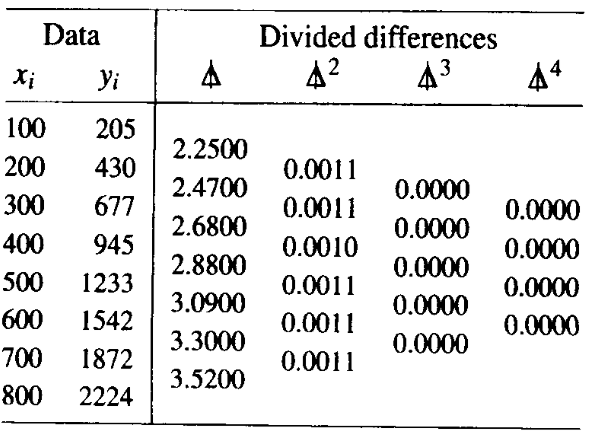
\includegraphics[width=.5\textwidth{}]{record-dif.png}
    \caption{录音机数据的均差表}
  \end{figure}

  可以看到,二阶均为常数,三阶均差到小数点后4位均为0,可以看出数据基本是二次的,可以用二次多项式作为经验模型.
  
\end{frame}

\begin{frame}{差分表中的观测值}

  \begin{itemize}
  \item 对“小”的评判是相对的、定性的.
  \item 必须灵敏地感觉数据中出现的误差和不规则变化.
  \end{itemize}
  
\end{frame}

\begin{frame}{车辆的停止距离}
  \begin{figure}
    \centering{}
    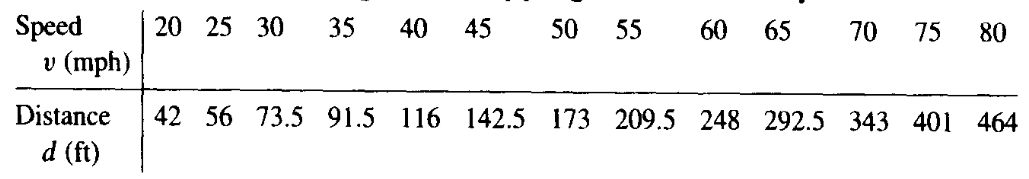
\includegraphics[width=.7\textwidth{}]{car-tab.png}
  \end{figure}
  \begin{figure}
    \centering{}
    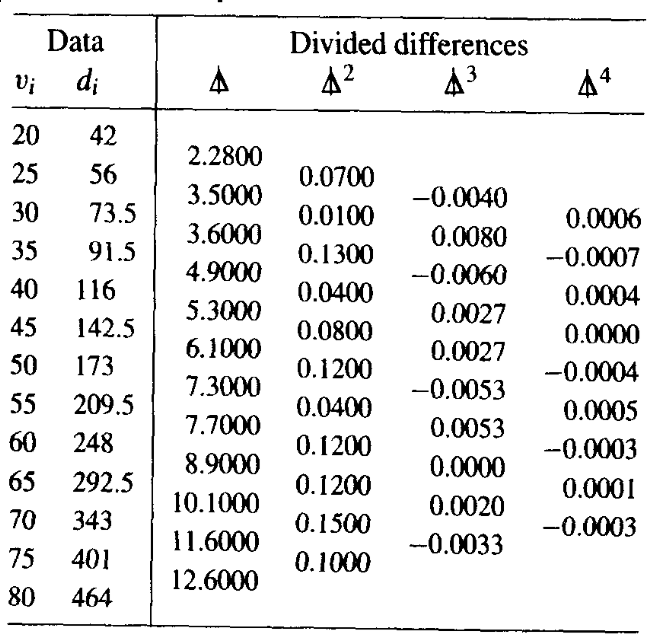
\includegraphics[width=.5\textwidth{}]{car-dif.png}
  \end{figure}
\end{frame}

\begin{frame}{用二阶模型进行拟合}
  \[
  P(v) = a + bv + cv^2
  \]
  用最小二乘法求解:
  \[
  \text{Minimize } S = \sum_{i=1}^m [d_i - (a + bv_i + cv_i^2)]^2
  \]
  存在极小点的必要条件$\frac{\partial S}{\partial a} = \frac{\partial S}{\partial b} = \frac{\partial S}{\partial c} = 0$, 故
  \[
  ma + (\sum v_i)b + (\sum v_i^2)c = \sum d_i
  \]
  \[
  (\sum v_i)a + (\sum v_i^2)b + (\sum v_i^3)c = \sum v_id_i
  \]
  \[
  (\sum v_i^2)a + (\sum v_i^3)b + (\sum v_i^4)c = \sum v_i^2d_i
  \]

\end{frame}

\begin{frame}{模型验证}
  \[
  P(v) = 50.0594 - 1.9701v + 0.0886v^2
  \]

  \begin{figure}
    \centering{}
    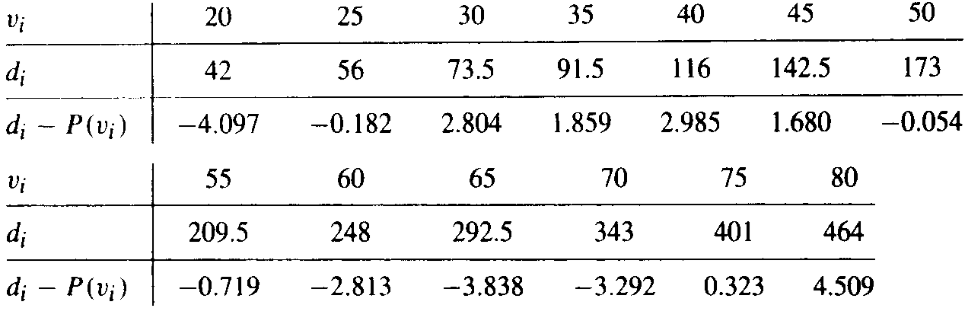
\includegraphics[width=.7\textwidth{}]{car-comp.png}
    \caption{用二次多项式光滑化停止距离}
  \end{figure}

  当$v = 0$时呢?

\end{frame}

\begin{frame}{酵母培养物的增长}

  \begin{figure}
    \centering{}
    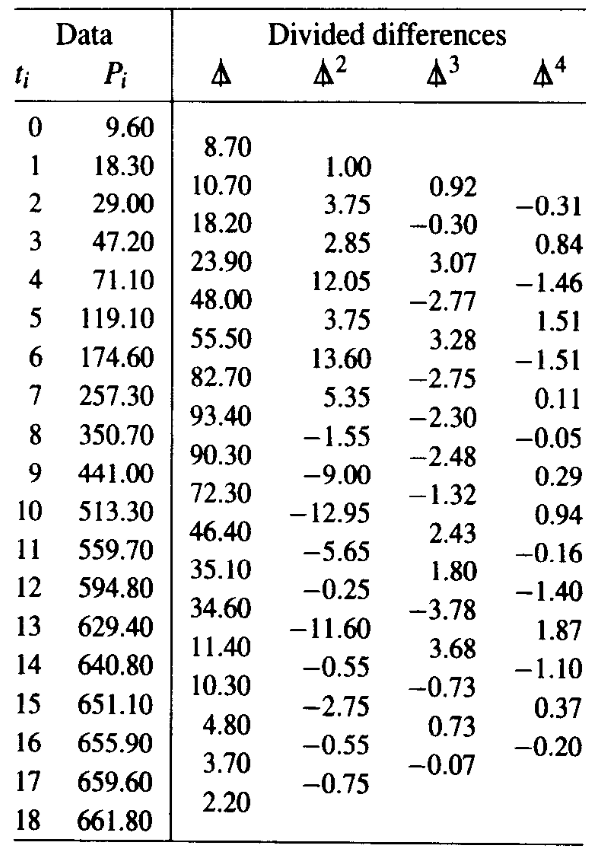
\includegraphics[height=.7\textheight{}]{yeast-tab.png}
    \caption{差分表}
  \end{figure}
  
\end{frame}

\begin{frame}{拟合结果}
  \[
  P = -93.82 + 65.70t -1.12t^2
  \]

  \begin{figure}
    \centering{}
    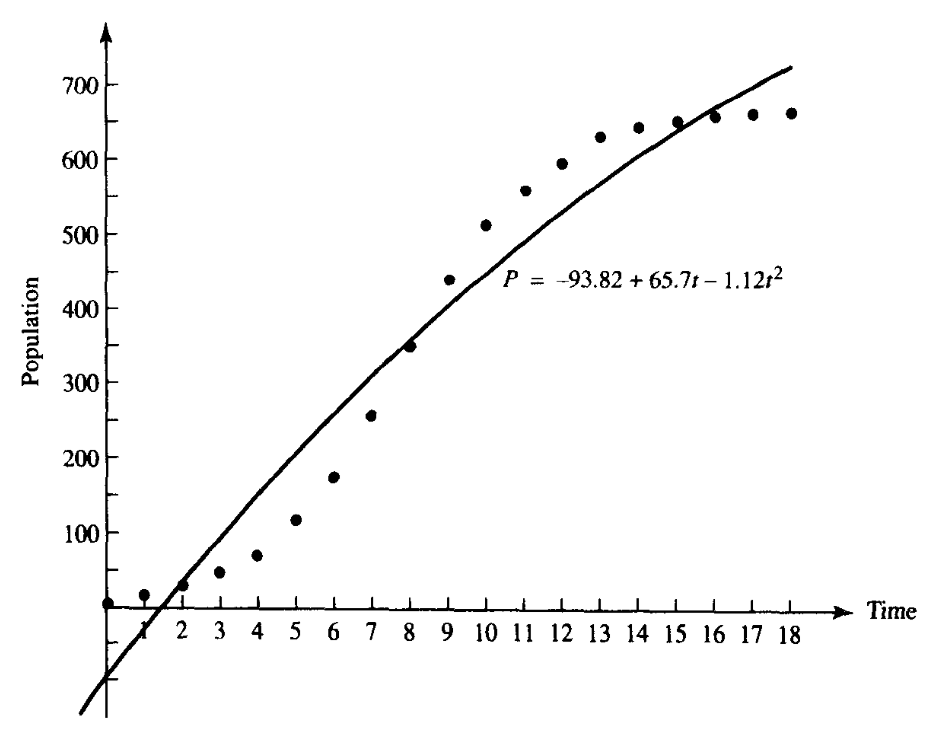
\includegraphics[height=.55\textheight{}]{yeast-fig.png}
  \end{figure}
  拟合失败!
  
\end{frame}

\begin{frame}{三阶样条模型}

  在连续的数据点对间使用不同的三阶多项式,追踪数据的趋势.

  \begin{description}
  \item[高阶多项式] 端点处有摆动倾向,对数据中小的变化太敏感
  \item[低阶多项式] 拟合效果不好(如速度很快时的刹车问题模拟)
  \item[三阶样条插值] 既保证基本关系的特征,同时减少摆动的倾向和数据变换的敏感性
  \end{description}
  \begin{figure}
    \centering{}
    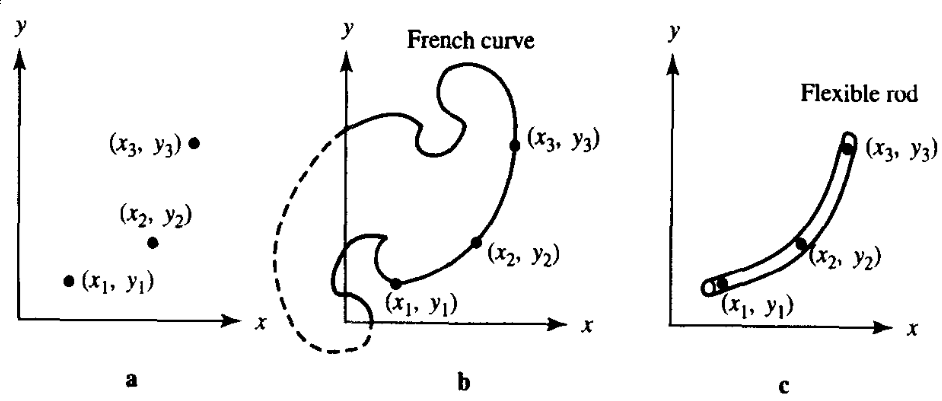
\includegraphics[width=.7\textwidth{}]{spline.png}
  \end{figure}
  
\end{frame}

\begin{frame}{线性样条}
  \begin{figure}
    \centering
    \setcounter{subfigure}{0}{}
    \subfloat[线性样条是含直线段的连续函数]{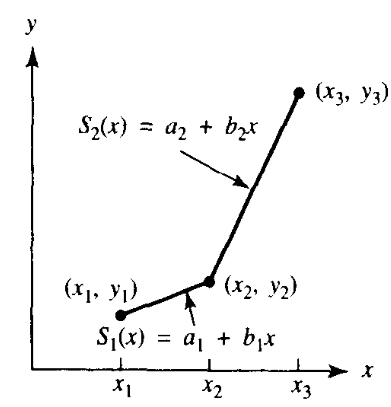
\includegraphics[height=.5\textheight{}]{line-spline.png}}
    \subfloat[由于一阶导数不连续,线性样条不光滑]{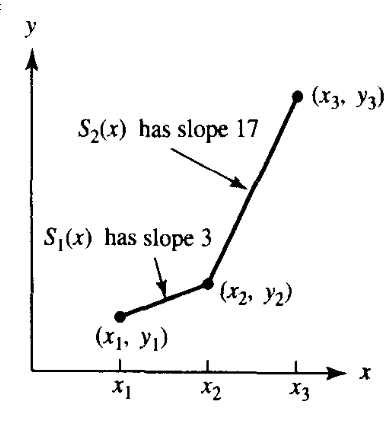
\includegraphics[height=.5\textheight{}]{line-spline-slope.png}}
  \end{figure}
  
\end{frame}

\begin{frame}{三阶样条}
  \begin{figure}
    \centering{}
    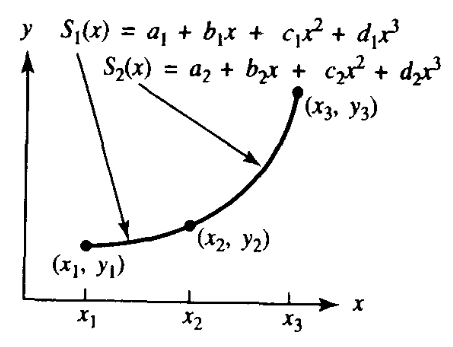
\includegraphics[width=.4\textwidth{}]{cubic-spline.png}
  \end{figure}
  \[
  S_1(x) = a_1 + b_1x + c_1x^2+d_1x^3, x \in [x_1, x_2)
  \]
  \[
  S_2(x) = a_2 + b_2x + c_2x^2+d_2x^3, x \in [x_2, x_3)
  \]
  
\end{frame}

\begin{frame}{三阶样条求解}
  \[
  S_1'(x) = b_1 + 2c_1x+3d_1x^2, x \in [x_1, x_2)
  \]
  \[
  S_1''(x) = 2c_1+6d_1x, x \in [x_1, x_2)
  \]
  \[
  S_2'(x) = b_2 + 2c_2x+3d_2x^2, x \in [x_2, x_3)
  \]
  \[
  S_2''(x) = 2c_2+6d_2x, x \in [x_2, x_3)
  \]

  求解:
  \[
  S_1(x_1) = y_1
  \]
  \[
  S_1(x_2) = y_2
  \]
  \[
  S_2(x_2) = y_2
  \]
  \[
  S_2(x_3) = y_3
  \]
  
\end{frame}

\begin{frame}{约束条件}

  连接处导数约束: $S_1'(x_2) = S_2'(x_2)$, $S_1''(x_2) = S_2''(x_2)$

  端点约束(自然样条):$S_1''(x_1) = 0$, $S_2''(x_3) = 0$

  端点约束(强制样条):$S_1'(x_1) = f'(x_1)$, $S_2'(x_3) = f'(x_3)$

  \begin{figure}
    \centering{}
    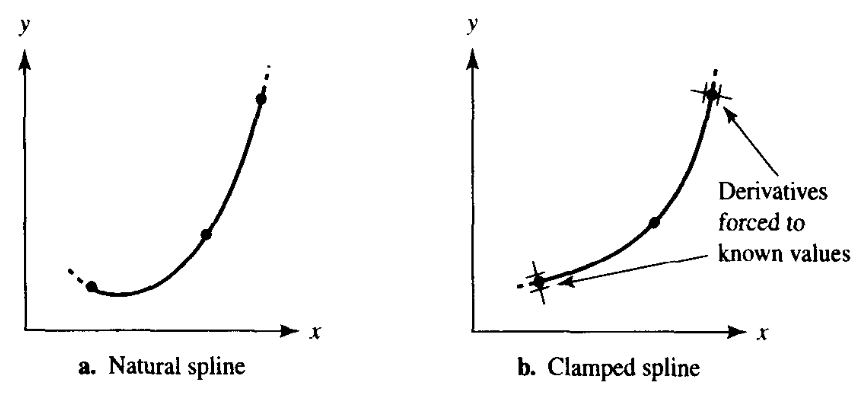
\includegraphics[width=.7\textwidth{}]{spline-border.png}
  \end{figure}
  
\end{frame}

\begin{frame}{拟合结果}
  \begin{figure}
    \centering{}
    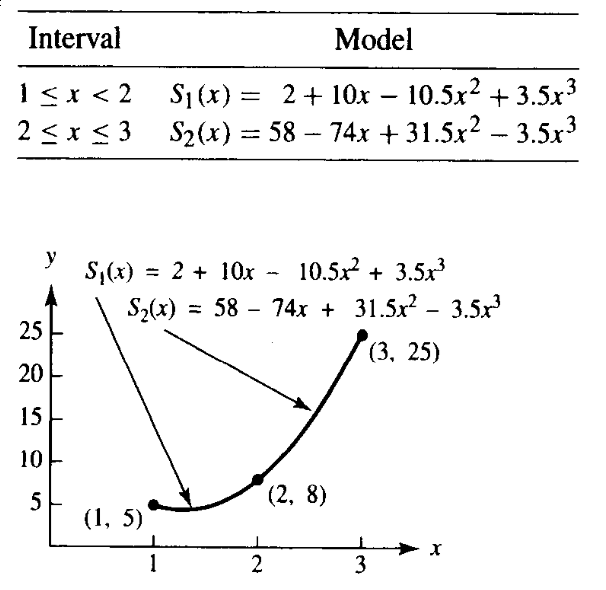
\includegraphics[width=.5\textwidth{}]{spline-fit.png}
  \end{figure}
  
\end{frame}

\begin{frame}{再论车辆的停止距离}
  \begin{figure}
    \centering{}
    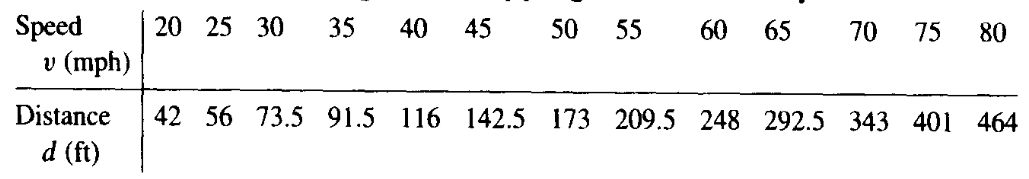
\includegraphics[width=.6\textwidth{}]{car-tab.png}
  \end{figure}

  \begin{figure}
    \centering{}
    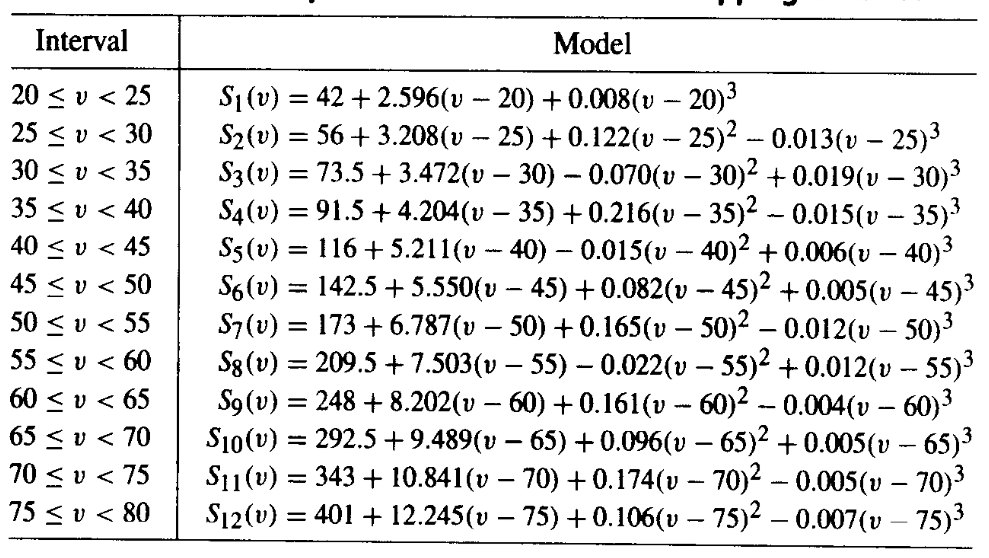
\includegraphics[width=.6\textwidth{}]{car-spline.png}
    \caption{三阶样条模型}
  \end{figure}

\end{frame}

\begin{frame}{拟合结果}
  \begin{figure}
    \centering{}
    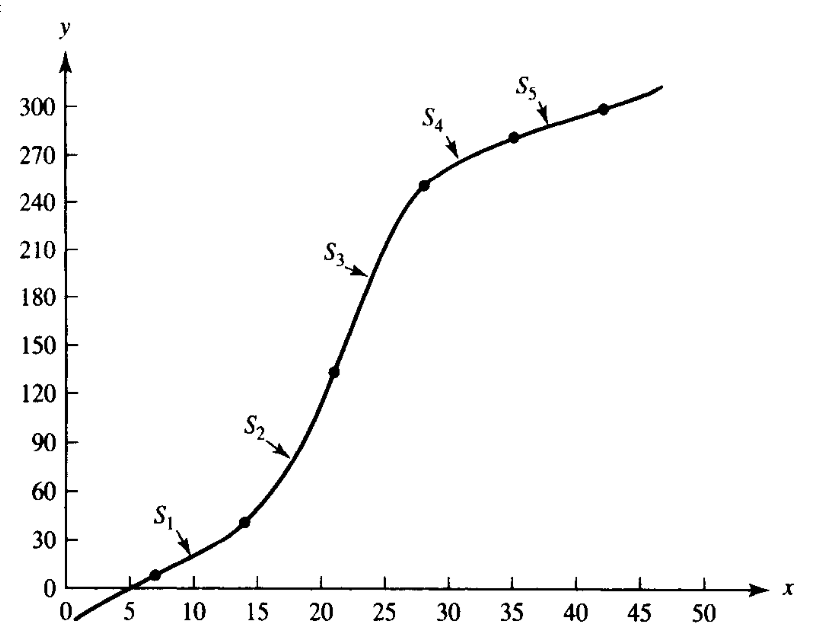
\includegraphics[width=.8\textwidth{}]{car-fit.png}
  \end{figure}
  

\end{frame}

\begin{frame}{构造经验模型}
  \begin{figure}
    \centering{}
    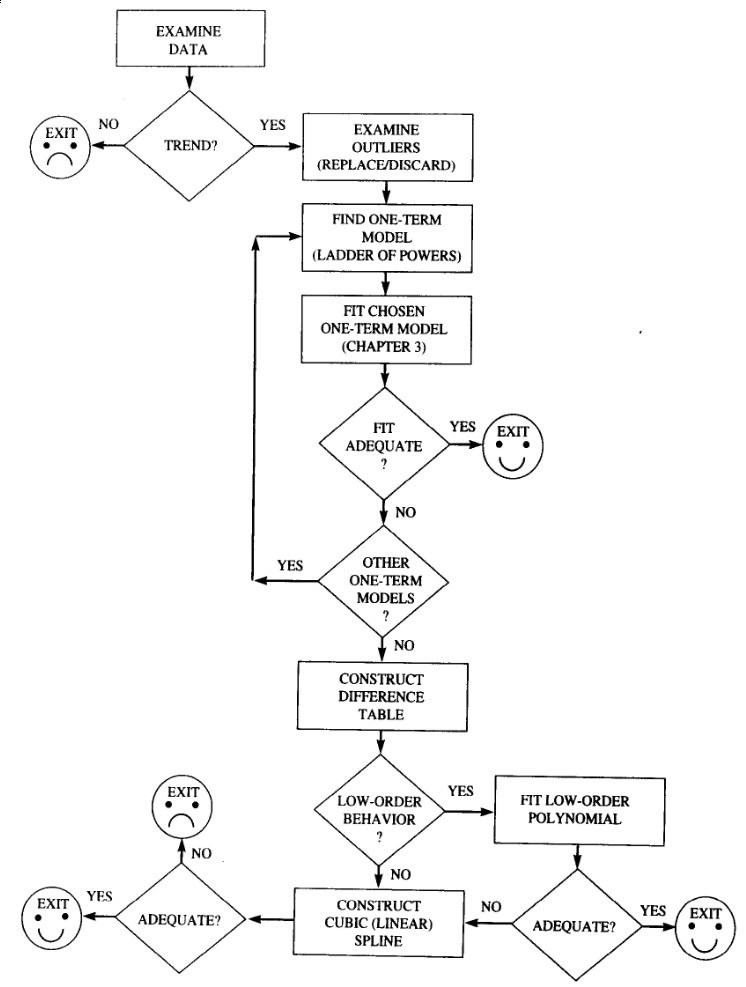
\includegraphics[height=.8\textheight{}]{model.png}
  \end{figure}

\end{frame}

\begin{frame}{作业}
  P123: 5
\end{frame}

\end{document}

%%% Local Variables: 
%%% TeX-master: t
%%% TeX-engine: xetex
%%% End: 
